47. \begin{figure}[ht!]
\center{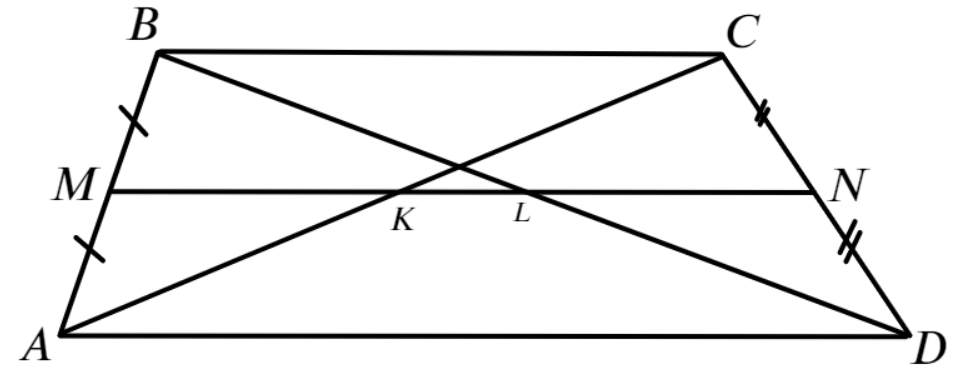
\includegraphics[scale=0.35]{g8-47.png}}
\end{figure}\\
Так как средняя линии трапеции $MN$ параллельна основаниям трапеции и проходит через середины $AB$ и $CD,$ отрезки $MK,\ KN$ и $LN$ также являются средними линиями в соответствующих треугольниках. Тогда $MN=\cfrac{1}{2}(12+18)=15$см, $MK=LN=\cfrac{1}{2}\cdot12=6$см, $KL=15-6-6=3$см.\\
